% Part: sets-functions-relations
% Chapter: relations
% Section: trees

\documentclass[../../../include/open-logic-section]{subfiles}

\begin{document}

\olfileid{sfr}{rel}{tre}
\olsection{వృక్షాలు}

తర్కశాస్త్రంలోని అన్ని భాగాలలో ముఖ్యమైన పాత్ర వహించే ఒక ప్రత్యేక
రకం పాక్షిక క్రమం \emph{వృక్షం}. ప్రాథమిక తర్కంలో పరిమిత వృక్షాలు
కనిపిస్తాయి. ఉదాహరణకు !!{formula}sను వాటి వాక్యనిర్మాణ వృక్షాలుగా
విభజించడం ద్వారా అర్థం చేసుకోవచ్చు. అలాగే అనేక !!{derivation}
వ్యవస్థలలో !!{derivation}s కూడా పరిమిత వృక్షాల రూపంలో ఉంటాయి.
%
ప్రవచన తర్కం, ప్రథమక్రమ తర్కం యొక్క సంపూర్ణతా సిద్ధాంతాల నిరూపణలలోనే
అనంత వృక్షాలు కనిపిస్తాయి; గణిత తర్కశాస్త్రమంతటా వాటిని ఉపయోగిస్తారు.

వృక్షం యొక్క సమితి-సిద్ధాంత భావనకు, గ్రాఫు సిద్ధాంతంలోని వృక్ష భావనతో
దగ్గరి సంబంధం ఉంది. ఒక పరిమిత వృక్షం చిత్రం ఇది:

\begin{center}
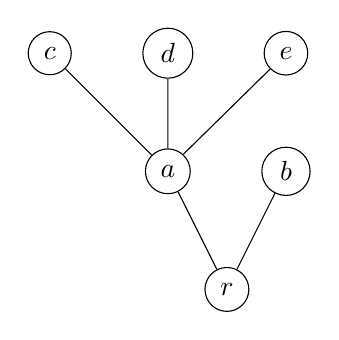
\begin{tikzpicture}[nodes={draw, circle}, -]
\node{$r$} [grow'=up]
    child { node {$a$} 
        child { node {$c$} }
        child { node {$d$} }
        child { node {$e$} }
    }
    child { node {$b$} };
\end{tikzpicture}
\end{center}

అన్నింటికంటే కింద ఉన్న శీర్షం $r$ వృక్షమూలం.
$r$ తప్ప ప్రతి శీర్షానికి దాని వెంటనే కింద కచ్చితంగా ఒక జనక శీర్షం ఉంటుంది.
$x$కు $y$తో ఉండే సంబంధాన్ని ఇలా చూడవచ్చు:
$x$ అనే శీర్షం నుంచి అంచులను అనుసరిస్తూ పైకి వెళ్లి $y$ అనే శీర్షాన్ని
చేరగలిగితే, $x$ను $y$ యొక్క \emph{పూర్వజంగా} పరిగణించవచ్చు.

వృక్షంలోని పూర్వజ సంబంధం ఒక కఠిన పాక్షిక క్రమం.
ఇదే సమితి-సిద్ధాంత నిర్వచనానికి ప్రేరణ.
దానిని చెప్పడానికి రెండు భావనలు కావాలి.
$\le$ ద్వారా పాక్షికంగా క్రమీకరించిన $A$ సమితిలో
\emph{కనిష్ఠ మూలకం} అంటే, ప్రతి $y \in A$కూ $x \le y$
అయ్యే !!a{element} $x \in A$.
ఒక సమితి యొక్క ప్రతి అశూన్య ఉపసమితికీ కనిష్ఠ మూలకం ఉంటే,
ఆ సమితి $\le$ ద్వారా \emph{సుక్రమీకరించబడింది} అంటాం.

\begin{defn}[వృక్షం]
ఒక \emph{వృక్షం} అంటే $T = \tuple{A, \le}$ అనే జత.
ఇక్కడ $A$ ఒక సమితి; $\le$ అనేది $A$పై పాక్షిక క్రమం.
దానికి ఏకైక కనిష్ఠ మూలకం $r \in A$ ఉంటుంది
(దీనిని \emph{వృక్షమూలం} అంటాం).
అలాగే ప్రతి $x \in A$కూ $\Setabs{y}{y \le x}$ అనే సమితి
$\le$ ద్వారా సుక్రమీకరించబడాలి.
\end{defn}

\begin{defn}[ఉత్తరవర్తులు]
$T = \tuple{A, \le}$ ఒక వృక్షం అనుకుందాం.
$x,y \in A$, $x < y$ అయి, $x < z < y$ అయ్యే $z \in A$
ఏదీ లేకపోతే, $y$ను $x$ యొక్క \emph{ఉత్తరవర్తి} అంటాం.
\end{defn}

$x \in A$ యొక్క ఉత్తరవర్తులను దాని \emph{సంతాన శీర్షాలు} అని కూడా అంటాం.
$y$ అనేది $x$ యొక్క ఉత్తరవర్తి అయితే, $x$ను $y$ యొక్క
\emph{పూర్వవర్తి} లేదా \emph{జనక శీర్షం} అంటాం.

\begin{prop}
$\tuple{A,\le}$ ఒక వృక్షం అయితే, వృక్షమూలం తప్ప ప్రతి
$x \in A$కూ గరిష్ఠంగా ఒక పూర్వవర్తి ఉంటుంది.
\end{prop}

\begin{proof}
  $y_1 < x$, $y_2 < x$, $y_1 \neq y_2$ అనుకుందాం.
  అప్పుడు $\{y_1, y_2\} \subseteq \Setabs{z}{z<x}$.
  $\Setabs{z}{z<x}$ అనేది $\le$ ద్వారా సుక్రమీకరించబడింది కనుక,
  దాని ఉపసమితి $\{y_1, y_2\}$కు కనిష్ఠ మూలకం ఉంటుంది.
  అది తప్పక $y_1$ లేదా $y_2$ అయి ఉండాలి.
  కనుక $y_1 \le y_2$ లేదా $y_2 \le y_1$.
  $y_1 \neq y_2$ అనుకున్నాం కనుక, నిజానికి $y_1 < y_2$
  లేదా $y_2 < y_1$. అలాగే $y_1 < x$, $y_2 < x$ అనుకున్నాం కనుక
  $y_1 < y_2 < x$ లేదా $y_2 < y_1 < x$.
  అందువల్ల $y_1$, $y_2$ రెండూ $x$ యొక్క పూర్వవర్తులు కాలేవు.
\end{proof}

\begin{defn}
$A$ అనంత సమితి అయితే $T = \tuple{A, \le}$ అనే వృక్షాన్ని
\emph{అనంత} వృక్షం అంటాం; లేకపోతే \emph{పరిమిత} వృక్షం అంటాం.
$T$లో ప్రతి $x \in A$కూ పరిమిత సంఖ్యలోనే ఉత్తరవర్తులు ఉంటే,
$T$ \emph{పరిమిత శాఖీకరణం} గల వృక్షం అంటాం.
\end{defn}

\begin{defn}[శాఖలు]
$T = \tuple{A, \le}$ అనే వృక్షంలో, $T$ యొక్క \emph{శాఖ}
అంటే $T$లో ఒక గరిష్ఠ శృంఖల.
అంటే $B \subseteq A$ అనే సమితి ఈ షరతులను సంతృప్తిపరచాలి:
ఏ $x, y \in B$కైనా $x \le y$ లేదా $y \le x$;
అలాగే ప్రతి $z \in X \setminus B$కూ,
$z \le u$, $u \le z$ రెండూ కాని $u \in B$ ఉండాలి.
%
$T$ యొక్క శాఖలన్నింటి సమితిని సూచించడానికి $[T]$ను ఉపయోగిస్తాం.
\end{defn}

\begin{ex}
పరిమిత శాఖీకరణం గల వృక్షానికి ఒక ప్రసిద్ధ ఉదాహరణ,
$0$లు, $1$ల పరిమిత క్రమాలతో ఏర్పడే \emph{అనంత ద్విసంకేత వృక్షం}.
దీనిని కొన్నిసార్లు $\{0,1\}^*$ లేదా $\Bin^*$ అని సూచిస్తారు;
ఇది పొడిగింపు సంబంధం $\sqsubseteq$ ద్వారా క్రమీకరించబడుతుంది
(ఉదాహరణకు $101 \sqsubseteq 101101$).
ఏ ద్విసంకేత సంకేతమాల చివరనైనా $0$ లేదా $1$ను చేర్చి ఎప్పుడూ
పొడిగించవచ్చు కనుక, ఈ వృక్షంలో అనంతంగా మూలకాలు ఉంటాయి:
ప్రతి మూలకం $s$కూ కచ్చితంగా రెండు ఉత్తరవర్తులు $s0$, $s1$ ఉంటాయి.
దీని వృక్షమూలం శూన్య క్రమమైన $\emptyseq$.
\end{ex}

\begin{ex}
ఇంకొంచెం సాధారణంగా, సహజ సంఖ్యల పరిమిత క్రమాల సమితి $\Nat^*$ కూడా,
పొడిగింపు సంబంధం $\sqsubseteq$తో కలిపి, ఒక వృక్షం.
ఇది పరిమిత శాఖీకరణం గలది కాదని స్పష్టం: ప్రతి $s \in \Nat^*$కూ,
ఒక్కో $n \in \Nat$కు ఒక్కొక్కటి చొప్పున, అనంతంగా $sn$ ఉత్తరవర్తులు ఉంటాయి.
$\sqsubseteq$ కింద సంవృతమైన ప్రతి $A \subseteq \Nat^*$,
$\Nat^*$ యొక్క \emph{ఉపవృక్షం}.
(అంటే $s \in A$, $s' \sqsubseteq s$ అయితే $s' \in A$ కూడా అయ్యేలా
$A$ ఉండాలి.) పరిమిత వృక్షాలన్నింటినీ $\Nat^*$ యొక్క పరిమిత
ఉపవృక్షాలుగా సూచించవచ్చు.
\end{ex}

\begin{prop}[కోనిగ్ ఉపసిద్ధాంతం]
$T = \tuple{A,\le}$ అనేది పరిమిత శాఖీకరణం గల అనంత వృక్షం అయితే,
$T$కు ఒక అనంత శాఖ ఉంటుంది.
\end{prop}

గణనీయతా సిద్ధాంతంలో విస్తృతంగా ఉపయోగించే కోనిగ్ ఉపసిద్ధాంతంలోని
ఒక ప్రత్యేక సందర్భాన్ని \emph{బలహీన కోనిగ్ ఉపసిద్ధాంతం} అంటారు.
అది: $\{0,1\}^*$ యొక్క ఏ అనంత ఉపవృక్షానికైనా ఒక అనంత శాఖ ఉంటుంది.

\end{document}
